\subsection{Energy and Mass} 

(Answers to M\Alph{subsection} problems are on page \pageref{energy_mass_prob_answers}.)


\begin{Exercise}[difficulty=1]
\label{problem_ball_and_cliff_basic}
Anna and Bob, curious about conservation of energy, head to a 10-meter-high cliff, armed with a 4~kg bowling ball.  Bob drops the bowling ball from the top of the cliff; as it falls, 392 joules of gravitational potential energy are converted to kinetic energy $K$ of the bowling ball.  What is the final speed of the ball at the bottom of the cliff, just before it hits the ground?
\end{Exercise}
\begin{Answer}
14 m/s
\end{Answer}

\begin{Exercise}[difficulty=1]
\label{problem_ball_and_cliff_trampoline}
Anna and Bob decide to drop the bowling ball off the cliff again, as they did in 
Problem~\ref{problem_ball_and_cliff_basic}.  This time, Anna places a large trampoline at the bottom of the 10-meter cliff, and Bob drops the bowling ball so that it lands directly on the trampoline.  The ball depresses the center of the trampoline and then bounces back up roughly to Bob's height.  Anna notices that when the bowling ball is at its lowest point, the springs on the edges of the trampoline are all visibly stretched.  How much potential energy is stored in the springs at the moment when they are at their maximum stretch?
\end{Exercise}
\begin{Answer}
392 J
\end{Answer}


\begin{Exercise}[difficulty=0]
Anna and Bob do one final experiment at the same cliff in Problems~\ref{problem_ball_and_cliff_basic} and \ref{problem_ball_and_cliff_trampoline}.  At the top of the cliff, instead of simply dropping the ball, Bob throws the ball directly downward, giving it an initial speed of $v_i=6$~m/s.  (a)~How much kinetic energy did Bob add to the bowling ball with his throwing motion?  (b)~What is the final velocity of the ball at the bottom of the cliff, just before it hits the ground (or the trampoline)?
\end{Exercise}
\begin{Answer}
(a) 72 J (b) 15.2 m/s
\end{Answer}



\begin{Exercise}[difficulty=0]
\label{prob_K_at_low_and_high_speeds}
A helium atom has a mass of $m=6.68 \times 10^{-27}$~kg.  Use both the Newtonian expression $K=\frac{1}{2} mv^2$ and the relativistic expression $K=(\gamma -1)mc^2$ to calculate the kinetic energy of the helium atom (a)~at $v=0.008c$ (b)~at $v=0.08c$, and (c)~at $v=0.8c$.
\end{Exercise}
\begin{Answer}
(a)~$1.9238 \times 10^{-14}$~J, $1.9239 \times 10^{-14}$~J  
(b)~$1.9238 \times 10^{-12}$~J, $1.9331 \times 10^{-12}$~J  
(c)~$1.9238 \times 10^{-10}$~J, $4.008 \times 10^{-10}$~J
\end{Answer}


\begin{Exercise}[difficulty=0]
You've just seen in Problem~\ref{prob_K_at_low_and_high_speeds} that for low speeds ($v \ll c$), the Newtonian expression and the relativistic expression for kinetic energy yield similar results.  Now, you'll prove it.  (a)~Write the relativistic expression for kinetic energy $K$, but do so by writing out $\gamma$ in terms of $v$ and $c$.  (That is, just substitute in the equation for $\gamma$.)  (b)~Rewrite the relativistic expression for $K$ using an exponent of $-\frac{1}{2}$ rather than a square root sign, and use the binomial series expansion $(1+x)^\alpha \approx 1+\alpha x$ to expand $\gamma$.  (See Lab~\ref{binomial_expansion_lab}.  We'll assume here that $v/c \ll 1$, so that you only need to keep the first two terms of the expansion, ignoring anything of order $x^2$ or higher.)  (c)~Show that your result reduces to the Newtonian result~$K=\frac{1}{2} mv^2$.
\end{Exercise}


\begin{minipage}{0.60 \textwidth}
\begin{Exercise}[difficulty=0]
\label{prob_collision_2m_and_m}
Two particles of different masses collide together.  The first particle has a mass $2m$ and speed $u_1=0.5c$.  The second particle has a mass of $m$ (half the first mass) and a speed of $u_2=0.756c$ in the opposite direction.  When they collide and stick together, the resulting particle is at rest, with velocity $u_{\rm f}=0$.  (a)~What is the mass $M$ of the resulting particle?  (b)~How much kinetic energy is converted to mass during the collision?
\end{Exercise}
\end{minipage}
\begin{minipage}{0.39 \textwidth}
\hspace{\fill}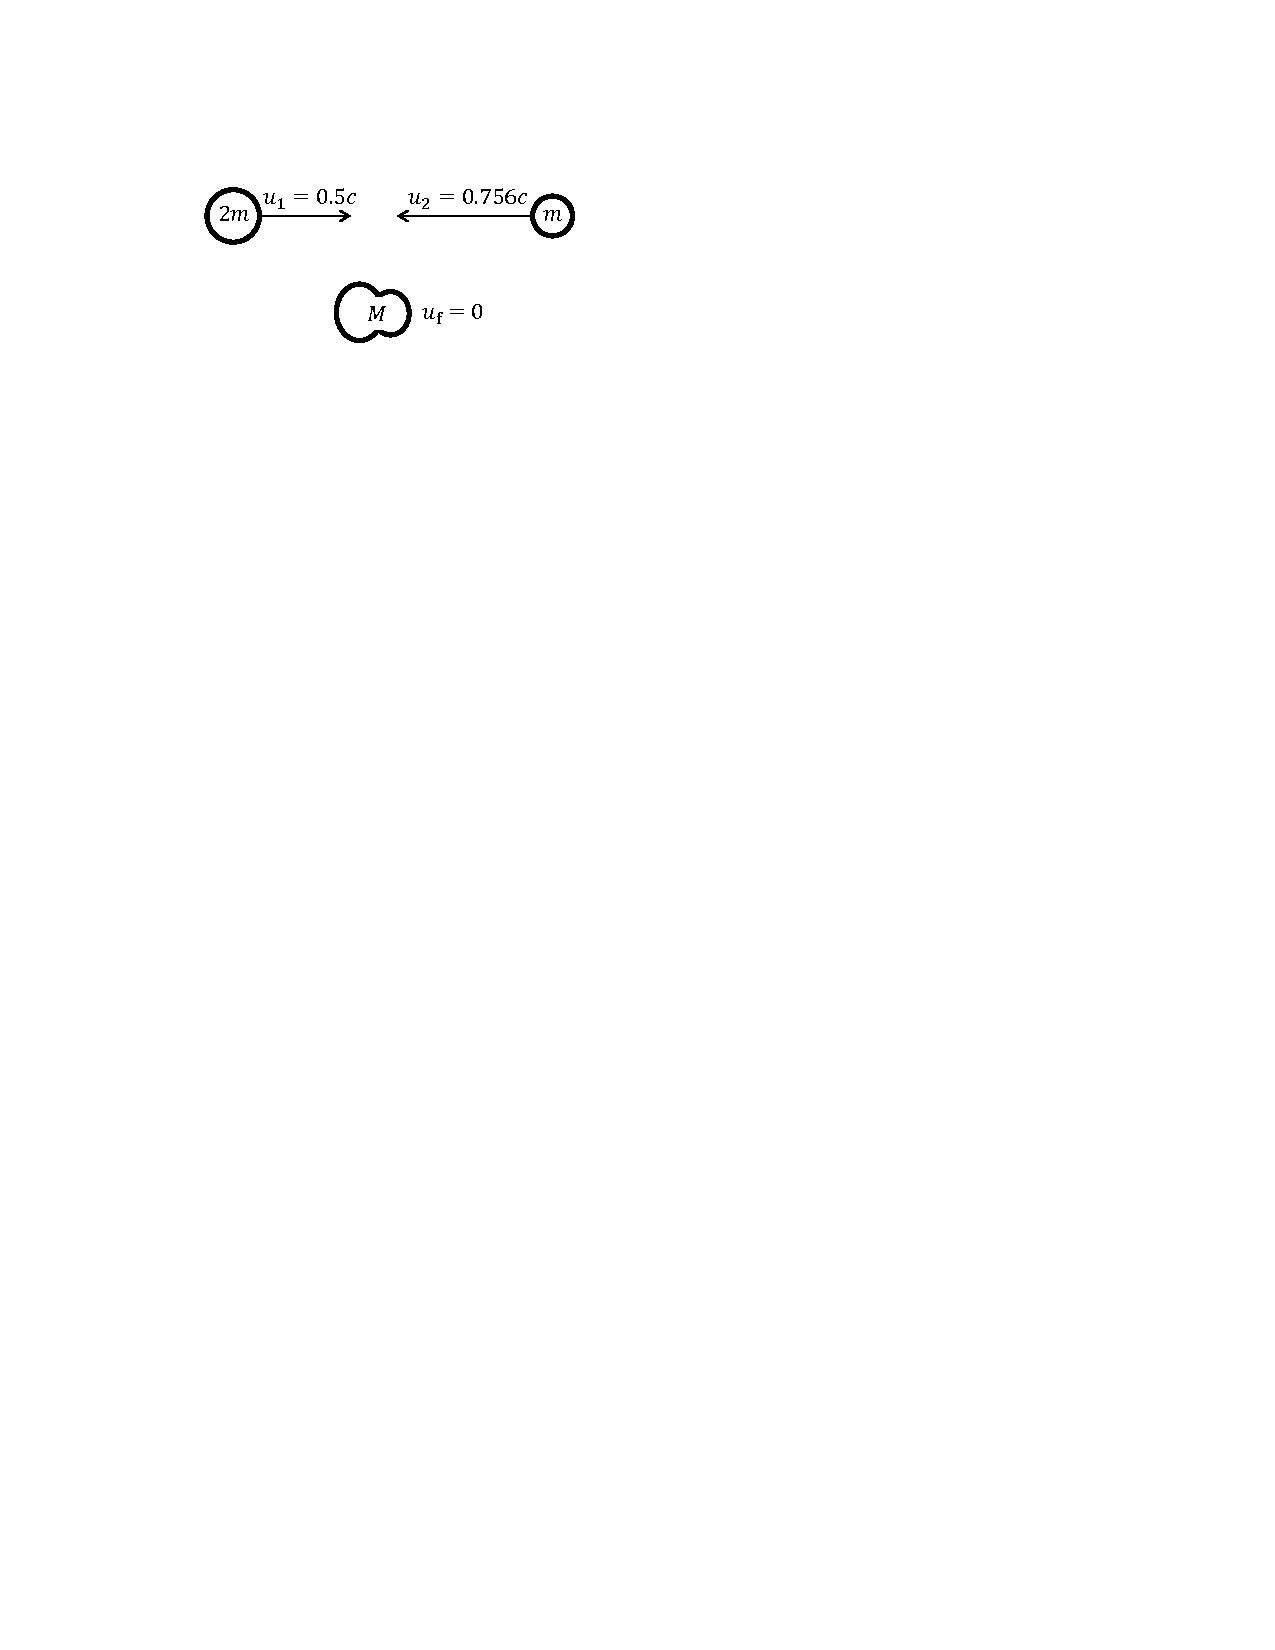
\includegraphics[scale=0.9]{M_problems/energy_mass/collision_m_and_2m.pdf}
\end{minipage}
\begin{Answer}
(a) $3.84m$ (b) $0.84mc^2$
\end{Answer}


\begin{Exercise}[difficulty=0]
In this problem, we'll analyze the collision of Problem~\ref{prob_collision_2m_and_m} in a reference frame with speed $v=0.5c$, in which the first particle now has speed $u_1=0$.  (a)~What are the speeds of the other original particle and the resulting particle in this reference frame?  (b)~What is the initial kinetic energy of the system before the collision?  (c)~What is the final kinetic energy of the system after the collision?  (d) What is the total energy $E_{\rm total}$ of the system in this reference frame?
\end{Exercise}
\begin{Answer}
(a) $0.911c$, $0.5c$ (b) $1.43mc^2$ (c) $0.59mc^2$ (d) $4.43mc^2$
\end{Answer}


\begin{Exercise}[difficulty=0]
In Problem \ref{problem_ball_and_cliff_trampoline}, Bob dropped a 4~kg bowling ball from a height of 10~meters onto a trampoline, visibly stretching its springs.  By how much did the mass of the springs change, and did they become heavier or lighter?
\end{Exercise}
\begin{Answer}
The springs' mass increases by $4.35 \times 10^{-15}$~kg.
\end{Answer}


\begin{minipage}{0.60 \textwidth}
\begin{Exercise}[difficulty=0]
In one of the common reactions late in a star's life cycle, nitrogen and hydrogen combine to produce one carbon atom and one helium atom:
$$
\isotope[15][7]{N} + \isotope[1][1]{H} \longrightarrow \isotope[12][6]{C} + \isotope[4][2]{He}.
$$
How much energy is given off by this reaction?  The table to the right lists the masses of each isotope in atomic mass units (amu), where $1~{\rm amu}=931.494~{\rm MeV}/c^2$.  (See Appendix~\ref{appendix_nuclear_primer} for an explanation of the isotope notation in the table.)
\end{Exercise}
\end{minipage}
\begin{minipage}{0.39 \textwidth}
\hspace{\fill}
{\renewcommand{\arraystretch}{1.5}
\begin{tabular}{|C{0.8in}|C{1.0in}|} \hline 
\textbf{Isotope} & \textbf{Mass (in amu)} \\ 
\hhline{|=|=|}
 \isotope[1][1]{H} & 1.007825 \\ \hline 
 \isotope[4][2]{He} & 4.002603 \\ \hline 
 \isotope[12][6]{C} & 12.0000000 \\ \hline 
 \isotope[15][7]{N} & 15.0001089 \\ \hline 
\end{tabular} }

\end{minipage}
\begin{Answer}
4.96 MeV
\end{Answer}


\begin{Exercise}[difficulty=0]
A typical large nuclear reactor produces about 1000 megawatts of electrical power, enough to power between 500,000 and 1,000,000 homes.  Over the course of a year, a reactor like that produces about $3 \times 10^{16}$~joules of energy.  Keeping it running requires about 30 metric tons (30,000~kg) of uranium, formed into pellets and stacked into fuel rods.  The rods are replaced every few years.  How much does the total mass of these rods change over the course of one year?  Do the rods become lighter or heavier?
\end{Exercise}
\begin{Answer}
The rods become lighter, by about a third of a kilogram.  Incidentally, a similarly-sized coal-burning plant burns more like 2,000,000 metric tons ($2 \times 10^9$~kg) of coal per year, most of which ends up as carbon dioxide in our atmosphere.
\end{Answer}




\bigskip\bigskip\bigskip
\pagebreak[3]
\textbf{Answers to Selected {\thesubsection} Problems:}
\label{energy_mass_prob_answers}
%\shipoutExercise
\shipoutAnswer

\cleardoublepage